\documentclass{article}
\usepackage[utf8]{inputenc}
\usepackage{graphicx}
\usepackage{geometry}

\geometry{
a4paper,
total={170mm,247mm},
left=20mm,
top=20mm}

\title{Systolic Array Specification}
\author{Vinod Ganesan, Gokulan Ravi}

\begin{document}

\maketitle
\section{Overview}
The systolic-array based accelerator is used to accelerate Deep Learning Inference. It acts as a peripheral device alongside the Shakti C-Class processor. The accelerator is completely parameterized, hence is easily extensible. The entire accelerator is written in Bluespec System Verilog (BSV), a high-level hardware description language.

\section{Packages}

\subsection{intMul\_WS}

\begin{figure}
  \centering
  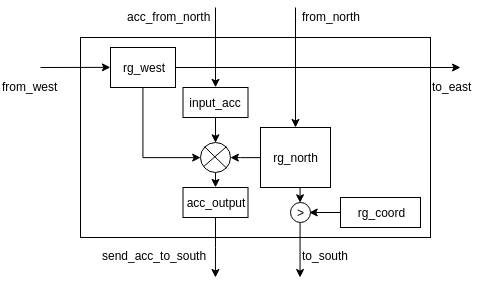
\includegraphics[scale=0.7]{./images/mkintMul_WS.png}
  \caption{mkintMul\_WS module, the smallest MAC unit}
  \label{fig:fig1}
\end{figure}

  \texttt{intMul\_WS} package provides module definition for the smallest \textbf{M}utiply-\textbf{AC}cumulate (MAC) unit or Processing Element (PE). It forms the building block of systolic array. The module \texttt{mkintMul\_WS} is polymorphic, and so is the interface for the module, \texttt{Ifc\_intMul\_WS}. 

\begin{verbatim}
module mkintMulWS#(Int#(8) row, Int#(8) col, parameter Integer coord)(Ifc_intMul_WS#(bWidth))
    provisos(Mul#(bWidth, 2, twbWidth), Add#(a__, bWidth, twbWidth));
\end{verbatim}

The \texttt{x,y} coordinates of the PE in the systolic array is specified in the \texttt{row} and \texttt{column} parameters. \texttt{coord} parameter specifies the y-coordinate of the PE, to limit weight flow. An overview of the implementation is presented in Figure \ref{fig:fig1} . The systolic array is a M $\times$ N grid of PEs. The North-West corner is indexed (0,0) and other PEs are indexed accordingly. In a weight stationary dataflow, weights are populated from the North side, and traverse North to South. Inputs are populated from West side and traverse West to East. Accumulator values (outputs) are populated from North side, and traverse North to South. Hence, the following are the traversals of input, weight and output in a PE.

\begin{enumerate}
  \item \textbf{input:} Received from West through the \texttt{from\_west} interface, and sent to East by \texttt{to\_east} interface.
  \item \textbf{weight:} Received from North through \texttt{from\_north} interface, and sent to South by \texttt{to\_south} interface.
  \item \textbf{output:} Received from North through \texttt{acc\_from\_north} interface, and sent to South by \texttt{send\_acc\_to\_south} interface.
\end{enumerate}

The \texttt{bWidth} parameter specifies the number of bits in each input/weight value. Number of bits in output is twice \texttt{bWidth}. The respective interfaces for input and output carry input and output values respectively. Interface for weight has three values - the weight value, the coordinate upto which the weight should traverse and a dummy opcode. When a weight is received by a PE, it is propagated to the PE in the South \texttt{only if} the coordinate received is greater than the y-coordinate of the PE.

\begin{verbatim}
interface Ifc_intMul_WS#(numeric type bWidth);
  interface Put#(Tuple3#((Maybe#(Bit#(bWidth))),Bit#(8),Bit#(2))) from_north;
  interface Put#(Maybe#(Bit#(bWidth))) from_west;
  interface Put#(Bit#(TMul#(2,bWidth)))  acc_from_north;
  interface Get#(Bit#(TMul#(2,bWidth)))  send_acc_to_south;  
  interface Get#(Tuple3#(Maybe#(Bit#(bWidth)),Bit#(8),Bit#(2))) to_south;
  interface Get#(Maybe#(Bit#(bWidth))) to_east;
endinterface
\end{verbatim}

\subsection{systolic}

This package contains \texttt{mksystolic} module, which implements a \texttt{nRow} $\times$ \texttt{nCol} (parameterized) systolic grid, with each element in the grid being a Processing Element (PE), an instance of \texttt{mkintMul\_WS} module. Taking care of edge conditions, each PE is connected with another PE in all four directions.

\begin{verbatim}
  module mksystolic(Ifc_systolic#(nRow,nCol,mulWidth))
      provisos (Add#(a__, mulWidth, TMul#(mulWidth, 2))); 
\end{verbatim}

In addition to \texttt{nRow} and \texttt{nCol}, the module takes in \texttt{mulWidth} parameter, which is used in the \texttt{bWidth} parameter for initializing every \texttt{mkintMul\_WS} module. Except PEs present in the edges \( Row 0, Row \texttt{nRow-1}, Column 0, Column \texttt{nCol}-1 \) every PE is connected to four other PEs present in the North, South, West and East directions. 

\begin{verbatim}
interface Ifc_RFIFO_Connections#(numeric type mulWidth);
  method Action send_rowbuf_value(Maybe#(Bit#(mulWidth)) value); 
endinterface

interface Ifc_CFIFO_Connections#(numeric type mulWidth);
  method Action send_colbuf_value(Tuple4#(Maybe#(Bit#(mulWidth)), 
    Bit#(TMul#(2,mulWidth)), Bit#(8),Bit#(2)) value);
  method Action send_acc_value(Bit#(TMul#(2, mulWidth)) accinput);
  method ActionValue#(Bit#(TMul#(2,mulWidth))) send_accumbuf_value;
endinterface

interface Ifc_systolic#(numeric type nRow, numeric type nCol,  
                        numeric type mulWidth);
  interface Vector#(nRow, Ifc_RFIFO_Connections#(mulWidth)) rfifo;
  interface Vector#(nCol, Ifc_CFIFO_Connections#(mulWidth)) cfifo;
endinterface
\end{verbatim}

Interface \texttt{Ifc\_RFIFO\_Connections} is a per-row interface, to send input values to the systolic array. It consists of  \texttt{send\_rowbuf\_value} method, which sends input values to the PEs in Column 0, using their respective \texttt{from\_west} interface. \texttt{Ifc\_CFIFO\_Connections} is a per-column interface - to send weights and to send \& receive output values. It comprises of three methods - \texttt{send\_colbuf\_value} to send weights, \texttt{send\_acc\_value} to send outputs and \texttt{send\_accumbuf\_value} to receive outputs.

\subsubsection{Internal Connections}
Considering a systolic array of size \texttt{nRow} $\times$ \texttt{nCol}. A PE with index (i, j) has the following connections.

\begin{itemize}
  \item \textbf{i=0}: \texttt{from\_north} and \texttt{acc\_from\_north} interfaces used in \texttt{cfifo[j].send\_colbuf\_value}.
  \item \textbf{j=0}: \texttt{from\_west} interface is used in \texttt{rfifo[i].send\_rowbuf\_value}.
  \item \textbf{i=nRow-1}: \texttt{send\_acc\_to\_south} interface is used in \texttt{send\_accumbuf\_value}.
  \item \textbf{i!=0 and i!=nRow-1}:
\end{itemize}

\begin{figure}
  \centering
  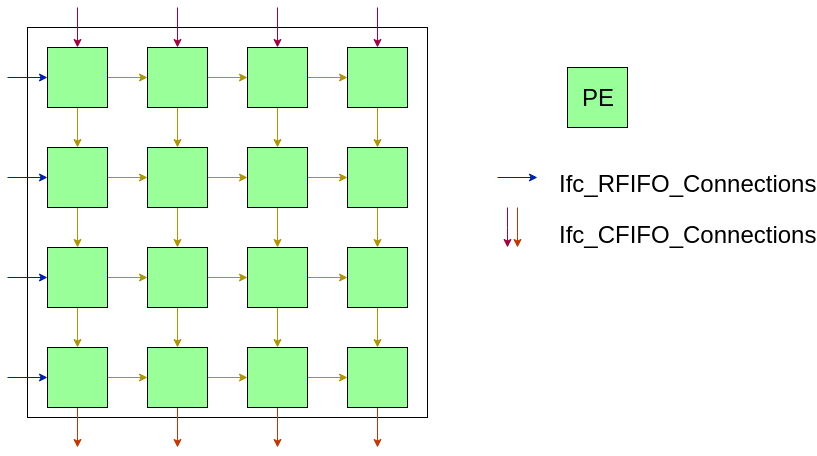
\includegraphics[scale=0.4]{./images/mksystolic.png}
  \caption{A 4 $\times$ 4 mksystolic module}
  \label{fig:fig1}
\end{figure}

\subsection{systolic\_top}

This package provides the module implementation for \texttt{mksystolic\_top\_axi4}, which acts as a peripheral alongside the processor. The module contains a AXI-4 slave module, which interacts with the \texttt{busWidth}-bit bus (64 for now). 

The module contains an instance of \texttt{mksystolic} module, to which inputs and weights are fed, and outputs are received from. When a \texttt{nRow} $\times$ \texttt{nCol} systolic array is initialized, we add additional FIFOs so that fetch and access can be separated. There are \texttt{nRow} FIFOs \(\texttt{rowBuffers}\), one per row, with each element of type \texttt{Bit\#\(mulWidth\)}. Also, there are \texttt{nCol} FIFOs, one per column, with each element of type \texttt{Tuple4\#(Bit\#(mulWidth), Bit\#(2*mulWidth), Bit\#(8), Bit\#(2))}. Each \texttt{Ifc\_Rfifo\_Connections} interface from the \texttt{mksystolic} instance connects to each of the FIFO, and fetches value from it. Similarly, each \texttt{Ifc\_Cfifo\_Connections} interface connects to each of the FIFO (\texttt{columnBuffers}), and fetches value from it. 

The module also contains two buffers - Global Buffer, Accumulator Buffers and a set of configuration registers. Global Buffer is used for storing input values. Accumulator buffer is used for storing accumulator values. Every input/weight received from the bus is stored in these buffers. Configuration registers are used to set convolution parameters like input dimensions, weight dimensions, padding. In addition to that, few registers act as control signals for systolic array to start or stop execution. All three units - Global Buffer, Accumulator buffer and Configuration registers, are memory-mapped.

\begin{verbatim}
module mksystolic_top_axi4(Ifc_systolic_top_axi4#(addr_width,data_width,user_width,
                          sqrtnRow,sqrtnCol,gbufaddr,accumaddr,nFEntries,mulWidth));
endmodule
\end{verbatim}

The following are the parameters for the polymorphic \texttt{mksystolic\_top\_axi4} module.
\begin{enumerate}
  \item \texttt{addr\_width}: Not used yet.
  \item \texttt{data\_width}: AXI-4 bus width.
  \item \texttt{user\_width}: Not used yet.
  \item \texttt{sqrtnRow}: Square-root of number of rows in the systolic array.
  \item \texttt{nCol}: Number of columns in the systolic array.
  \item \texttt{gbufaddr}: Number of bits used to index into an entry in the Global buffer.
  \item \texttt{abufaddr}: Number of bits used to index into an entry in the Accumulator buffer.
  \item \texttt{nFEntries}: Number of entries in each of the \texttt{rowBuffer} and \texttt{columnBuffer} FIFOs. 
  \item \texttt{mulWidth}: Number of bits in each input/weight. The same is used to initialize \texttt{mksystolic} module.
\end{enumerate}

\begin{verbatim}
interface Ifc_systolic_top_axi4#(numeric type addr_width, numeric type data_width, 
                                numeric type user_width, numeric type nRow, numeric type nCol, 
                                numeric type accumaddr,numeric type gbufaddr,  
                                numeric type nFEntries,numeric type mulWidth);
    interface AXI4_Slave_IFC#(`PADDR,data_width,0) slave_systolic;
    endinterface
\end{verbatim}

Number of banks in the \texttt{columnBuffer} should be the same as the number of columns in the systolic array. Since there are \texttt{nCols} number of columns, each column producing one output value per cycle, each value would be written to corresponding bank each cycle.

However, number of banks in the \texttt{rowBuffer} should be square-root of the number of rows in the systolic array. For example, with a $3 \times 3$ weight, each input value will be multiplied by three different input values, for three different continous outputs. Hence, if the unrolled filter size is of size \texttt{sqrtnRow * sqrtnRow}, it will be multiplied by \texttt{sqrtnRow} different continous weights, which would be populated in different continous rows. Hence Global buffer contains \texttt{sqrtnRow} banks, and each value is sent to \texttt{sqrtnRow} banks in the same number of cycles, each time to a different row.

The memory map of different memory units is listed below.
\begin{table}[h]
\begin{tabular}{|l|l|l|} \hline
Hardware                & Description                 & Address range           \\ \hline
Configuration Registers & IfmapDims                   & 'hB0000000              \\
                        & sysConfig                   & 'hB0000002              \\
                        & CoordCount                  & `hB0000004              \\
                        & weightCount                 & 'hB0000006              \\ \hline
Weights                 & WeightStart - WeightEnd     & 'hB0010000 - 'hB001ffff \\ \hline
Accumulator Buffer      & AccumBufStart - AccumBufEnd & 'hB0200000 - 'hB02fffff \\ \hline
Global Buffer           & GBufStart - GBufEnd         & 'hB0030000 - 'hB003ffff \\ \hline
\end{tabular}
\end{table}

\section{2D Convolution on systolic array}
The number of rows in the systolic array should be fixed as the number of elements when the weight is unrolled. Each column computes convolution of different filter. Firstly, configuration registers are set with input and weight dimensions. Then, all the weights are sent from the host processor and populated in the array through \texttt{ColumnBuffers}. Similarly all inputs are populated in Global buffer. The host sets the \texttt{startBit} register to start the systolic execution. Inputs are then sent to the systolic array through \texttt{rowBuffer} and output values are sent through \texttt{columnBuffers}. After all MAC operations complete, the output is finally stored in the Accumulator buffer, which is read by the host.
\end{document}
